%% This is an example first chapter.  You should put chapter/appendix that you
%% write into a separate file, and add a line \include{yourfilename} to
%% main.tex, where `yourfilename.tex' is the name of the chapter/appendix file.
%% You can process specific files by typing their names in at the 
%% \files=
%% prompt when you run the file main.tex through LaTeX.

\begingroup%
\makeatletter%
\cleardoublepage%
\let\newpage\relax%
\let\clearpage\relax%
\vspace*{\fill}%
\vspace*{\dimexpr-50\p@-\baselineskip}% Remove the initial
%% -default- 50pt gap (plus 1 line) 
\chapter{Conclusions and Directions for Further Research}
\label{chap5}
\vspace*{\fill}%
\endgroup%

\clearpage
Using a combination of field experiments, modeling approaches, geochemical analyses, and a new, high-throughput lipidomics method for identification of lipid biomarkers, this thesis examined the biogeochemical significance, in both absolute and relative terms, of various pathways of organic matter remineralization in the ocean. The results in \autoref{chap2} and \autoref{chap4} suggest that both biological and abiotic processes can augment or facilitate the degradation of organic matter by aerobic respiration at scales which are significant for ocean biogeochemistry. \autoref{chap3}, \autoref{chap4}, and \autoref{AppB} illustrate two ways in which lipids and their oxidation products can be combined as biomarkers to estimate the magnitude or significance of these processes.

As with any work of science, however, the findings in this thesis raise many more questions than they answer. Many of these questions center on the methods employed to reach these findings, and the various assumptions made. In this Conclusion, I briefly discuss the implications of some of these choices and offer some recommendations for future work in the relevant areas of research. If different values were assumed for conversion constants, or a different (non-normal) distribution was assumed for the population underlying some dataset, what additional (or different) insights might be gleaned from the same data? Or, for example, are there particular refinements that could be made to the data analysis methods employed in this thesis to open new avenues of discovery?

The results of Chapter 2 hinged on a number of assumptions discussed to varying degrees in the published manuscript. However, a reanalysis of the data --- or a similar future study --- might benefit from reconsideration of the size distribution of sinking particles and their resultant downward velocities. The average particle sinking velocities ($W_{avg}$) used throughout Chapter 2 and in most similar studies are assumed to represent the mean sinking velocities of populations of particles which are normally distributed in terms of size. However, there is considerable evidence (e.g., Alonso-Gonz\'{a}lez et al., 2010; Riley et al., 2012; Villa-Alfageme et al., 2014) that the size distribution of sinking marine particles in many systems is non-normal. If the model specified in \autoref{eq:c2e5} and \autoref{eq:c2e6} were reformulated to account for multiple particle size fractions, each with their own mean sinking velocities, one could use size-fractionated measurements of particle-attcached respiration to obtain estimates of \emph{k\textsubscript{S}}\textsubscript{,\emph{D},\emph{Z}} for each fraction. These estimates could then be used to assess the relative importance of various degradation processes within different reservoirs of particulate and colloidal organic matter.

In addition, one might expand or modify the approach in \autoref{chap2} to more fully account for temporal and spatial discontinuities that may exist between the supply and consumption of particulate organic matter in some marine systems. For example, the effect of vertically migrating zooplankton --- assumed to be negligible at the stations studied in this thesis --- can introduce spatial discontinuities between the mass balance sources and sinks implicit in such a model. In many systems, such as in the North Pacific Subtropical Gyre and Southern Ocean, zooplankton can transport large amounts of carbon across depths between the sea surface and mesopelagic ocean (Steinberg et al., 2008a; Steinberg et al., 2008b). Alternatively, in instances where the quantity of organic matter delivered to depth from the surface ocean far exceeds the capacity of the microbial population to metabolize it, significant temporal discontinuities may exist between sources and sinks. Several examples (Azam et al., 1994; Ducklow et al., 1993; Lancelot and Billen, 1984; Ortega-Retuerta et al., 2014) were discussed briefly in \autoref{ssec:Bacterial Production}, but such dynamics --- and the means by which they can be included in the types of models employed in this thesis --- warrant further consideration. To truly understand these lags and their effect, one would have to undertake a long-term study of particulate organic matter dynamics in a particular system at very high temporal resolution --- a logistically and financially daunting proposition, yet one which could be based on infrastructure already in place as a result of the National Science Foundation's Long Term Ecological Research (LTER) programs and Ocean Observatories Initiative (OOI).

\begin{SCfigure}[1][!t]
\centering
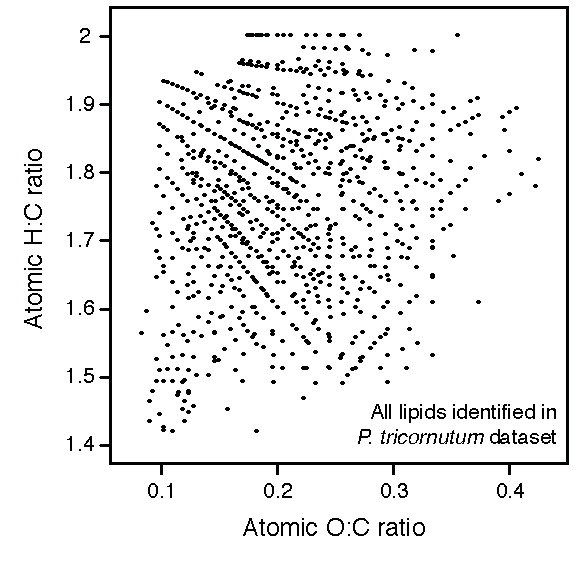
\includegraphics[width=.5\textwidth]{Fig_5-1.pdf}
\captionsetup{font={footnotesize}}
\caption[Basic Van Krevelen plot of the lipid data shown in \autoref{fig:c3n2}a]{Basic Van Krevelen plot of the lipid data shown in \autoref{fig:c3n2}a. Atomic O:C and H:C ratios of the various compounds were determined from elemental formulae.}
\label{fig:c5n1}
\end{SCfigure}

\begin{SCfigure}[1][!t]
\centering
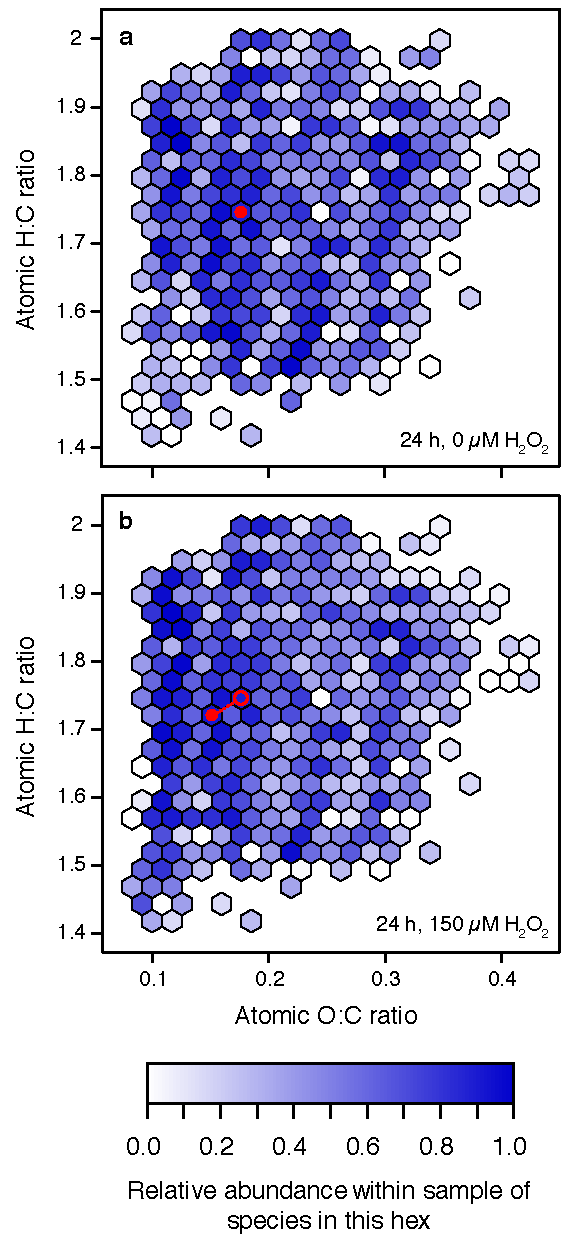
\includegraphics[width=.5\textwidth]{Fig_5-2.pdf}
\captionsetup{font={footnotesize}}
\caption[Hexagonal bin plots in Van Krevelen space of the data shown in \autoref{fig:c3n2}a and \autoref{fig:c5n1}]{Hexagonal bin plot in Van Krevelen space of the data shown in \autoref{fig:c3n2}b and \autoref{fig:c5n1}. Clustering of compounds into hexagonal bins preserves the integrity of the underlying data while reducing complexity to facilitate visual intepretation. (a) and (b) show the compounds identified in \emph{P. tricornutum} after 24 h in, respectively, the 0 $\mu$M H\textsubscript{2}O\textsubscript{2} control and 150 $\mu$M H\textsubscript{2}O\textsubscript{2} treatments. Color density indicates the relative abundance (via log transform and then normalization) of the identified lipid mass within each hex. The filled red symbols show the position in each sample of the bivariate median of the density field; the median position was determined by progressive erosion of hexes in each bin plot. The open red symbol in (b) shows the position of the median in (a), indicating a shift in bulk chemical composition of the \emph{P. tricornutum} lipidome toward the southwest under oxidative stress. This shift reflects the same major trends observed using the hierarchical clustering approach for which results are presented in \autoref{table:adn9} (i.e., apparent acyl elongation and an increase in acyl unsaturation under oxidative stress). Hexagonal binning and identification of the centroid via erosion were peformed using the hexbin package for R (Carr et al., 2015).}
\label{fig:c5n2}
\end{SCfigure}

The utility of the HPLC-MS data screening approach presented in \autoref{chap3} (i.e., \href{https://github.com/vanmooylipidomics/LOBSTAHS}{the LOBSTAHS software}) is limited in its current form by an incomplete understanding of the chemistry that determines the adduct formation hierarchies at the heart of the method. The default adduct ion hierarchies used to identify lipids in \autoref{chap3} and \autoref{chap4}, and \autoref{AppB} (i.e., those given in \autoref{table:adn2}) were determined empirically from repeated observations in the laboratory, and I recommend in \autoref{chap3} that other users of the software make their own empirical observations of formation patterns in all target lipid classes prior to commencing any analysis. However, a mechanistic understanding of the role of chemical structure in determining adduct ion formation patterns in different polar lipids would allow new users to predict hierarchies without direct observations. While relative and absolute adduct ion abundances are often reported in the literature, surprisingly little scientific attention has been given to the underlying chemistry that produces these patterns. This lack of attention is due in no small part to the fact that adduct formation --- and differences in response factors among the different adduct ions of the same precursor --- have been viewed largely as a nuisance to be minimized or a scientific transaction cost associated with HPLC-MS analysis. A few notable exceptions do exist, such as an excellent two-part study by Schug and McNair (Schug and McNair, 2002; 2003), who concluded that differences in adduct ion formation patterns between compounds could be explained by comparison of the acid dissociation constants (p\emph{K\textsubscript{a}}), octanol-water partition coefficients (\emph{K}\textsubscript{\emph{i}ow}) and surface activities of the analytes and the pH, concentration, and type of solvent system. The work by Schug and McNair could provide the basis for a more specific future study of adduct ion formation mechanisms in polar lipids, the results of which could be used to build a predictive tool within LOBSTAHS.

A second limitation of the current approach bears not on its design, but instead on how the hundreds of compounds that can be identified in a single sample are visualized and interpreted. For example, the data presented in \autoref{fig:c3n2} could be reexamined in a Van Krevelen ratio-ratio space, which would allow the user to begin associating changes between treatments with implied chemical mechanisms (\autoref{fig:c5n1}). However, trends can be difficult to discern in a ``simple'' Van Krevelen plot that contains $>$ 10\textsuperscript{3} features, as \autoref{fig:c5n1} illustrates. Alternatively, a hexagonal binning approach could be used to compare the results of different treatments in Van Krevelen space (\autoref{fig:c5n2}); clustering of compounds into hexagonal bins preserves the integrity of the underlying data while reducing complexity to facilitate visual interpretation. In \autoref{fig:c5n2}, the shift in Van Krevelen space of the multivariate median of the data under treatment with 150 $\mu$M H\textsubscript{2}O\textsubscript{2} (red symbol) is indicative of the same major trends that were observed in the \emph{P. tricornutum} experiment using the hierarchical clustering approach for which results are presented in \autoref{table:adn9} (i.e., apparent acyl elongation and an increase in acyl unsaturation under oxidative stress).

\begin{figure}[!th]
\centering
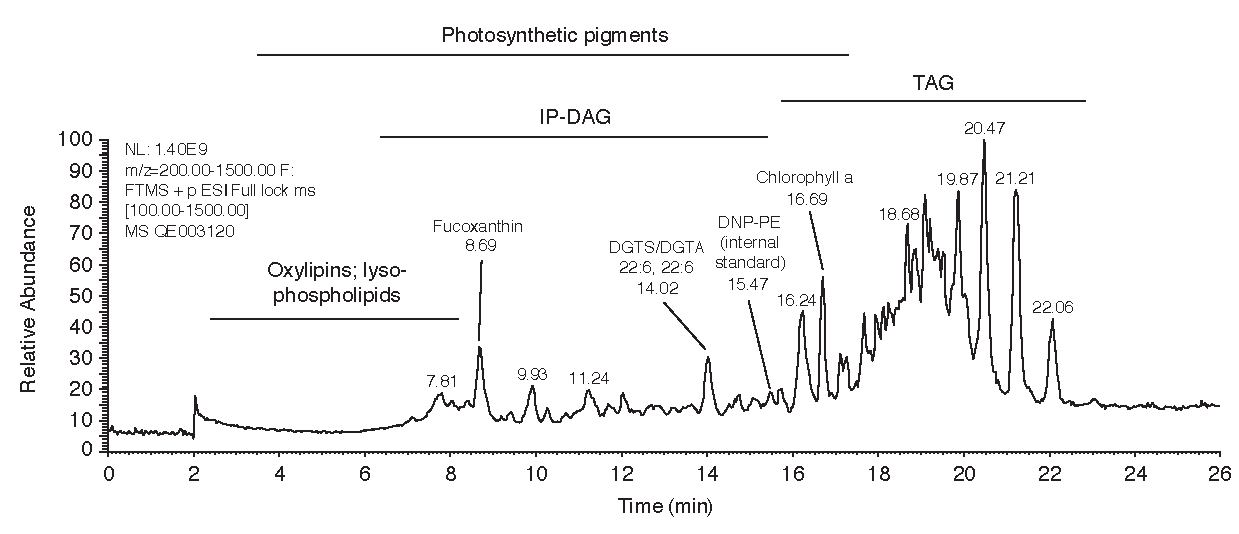
\includegraphics[width=1\textwidth]{Fig_5-3.pdf}
\captionsetup{font={footnotesize}}
\caption[Total ion current chromatogram of a typical marine lipid sample, with annotation of major features]{Total ion current chromatogram (all features, \emph{m/z} 200-1500, positive ionization mode) of a marine lipid sample typical of those described in \autoref{chap4} and \autoref{AppB}. Annotations show major features and retention time ranges for various classes of lipid . This figure shows the same water column sample from Station E, Arthur Habor, West Antarctica, which is presented in the leftmost position in \autoref{fig:c4n10} and \autoref{fig:c4n11}. HRAM-HPLC-ESI-MS analysis and subsequent identification and screening of lipids were performed as described in \autoref{chap4} and \autoref{AppE}.}
\label{fig:c5n3}
\end{figure}

Finally, the results presented in \autoref{chap3}, \autoref{chap4}, and \autoref{AppB} point to a more fundamental limitation of methods such as that described in \autoref{chap3}: The extent to which the mass spectral features in a given set of lipid data can be definitively characterized as individual compounds. One way to evaluate such methods is to examine the fraction of chromatographic peak area that can be identified by the method in a sample of typical complexity. Some performance statistics for the method described in \autoref{chap3} are given in \autoref{table:c3n2}; however, these are based on the number of mass spectral features present in the \emph{P. tricornutum} dataset at various stages of data analysis. Instead, \autoref{table:c5n1} shows the fractions of total chromatographic peak area in a typical environmental lipid sample from \autoref{chap4} (\autoref{fig:c5n3}) that were identified using LOBSTAHS at different levels of certainty. This accounting indicates that LOBSTAHS is capable in its current incarnation of identifying roughly half of the total peak area in the sample recorded for ions between 200 and 1500 \emph{m/z}. That roughly half of the total peak area remains unidentified in a typical sample --- as these results show --- is ample inspiration for improvements to the method. The HPLC-MS features in this unidentified fraction may very well represent additional compounds we would typically consider to be lipids. But it is well worth considering the nonselective nature of a lipid extraction, such as the modified Bligh and Dyer approach used throughout this work: The wide range of \emph{K}\textsubscript{\emph{i}ow} among natural organic compounds (Schwarzenbach et al., 2003) suggests many other hydrophobic molecules we typically do not consider to be lipids will likely almost always be present in the retained organic phase introduced into the mass spectrometer. The development of new methods to characterize this unidentified organic matter --- and improvements to current methods --- will continue to be a key focus of efforts in both biogeochemistry and human biochemistry.

In spite of these limitations, the results in this thesis --- particularly those in \autoref{chap4} and \autoref{AppB} --- demonstrate the potential of high-throughput lipid identification methods to assist biogeochemists and environmental scientists in assessing the impact of various processes and changes in marine ecosystems across a variety of spatial and temporal scales. The results in \autoref{chap4} indicate that changes and differences in ecosystem metalipidome composition can be used to assess shifts in microbial community structure and quantify the effect of various stressors on those communities. Based on this utility, one could make a strong case for the inclusion of such lipid data as a standard time-series measurement within the PAL-LTER and other LTER studies. A full exploitation of these molecules' potential in the context of the PAL-LTER study would require (1) a series of additional experiments to identify compounds diagnostic of various other sources of abiotic and biological stress and (2) characterization of the lipidomes of additional microorganisms important to the ecosystem, particularly those of the cryptomonads which have become an increasingly important component of spring and summer phytoplankton blooms. A commitment to sharing of data and a continuing emphasis on open-source software development will facilitate the production of both improvements and new methods that address these challenges.

\clearpage
\begin{singlespace}
\section*{References}
\addtocounter{section}{1}
{\setlength{\parindent}{0pt}
Alonso-Gonz\'{a}lez, I. J., J. Ar\'{i}stegui, C. Lee, A. Sanchez-Vidal, A. Calafat, J. Fabr\'{e}s, P. Sangr\'{a}, P. Masqu\'{e}, A. Hern\'{a}ndez-Guerra, and V. Ben\'{i}tez-Barrios (2010), Role of slowly settling particles in the ocean carbon cycle, \emph{Geophysical Research Letters}, \emph{37}(13), L13608, doi:\href{http://dx.doi.org/10.1029/2010GL043827}{10.1029/2010GL043827}.

{\setlength{\parskip}{10pt}

Azam, F., D. C. Smith, G. F. Steward, and \AA{}. Hagstr\"{o}m (1994), Bacteria-organic matter coupling and its significance for oceanic carbon cycling, \emph{Microbial Ecology}, \emph{28}(2), 167-179, doi:\href{http://dx.doi.org/10.1007/BF00166806}{10.1007/BF00166806}.

Ducklow, H. W., D. L. Kirchman, H. L. Quinby, C. A. Carlson, and H. G. Dam (1993), Stocks and dynamics of bacterioplankton carbon during the spring bloom in the eastern North Atlantic Ocean, \emph{Deep Sea Research Part II: Topical Studies in Oceanography}, \emph{40}(1-2), 245-263, doi:\href{http://dx.doi.org/10.1016/0967-0645(93)90016-G}{10.1016/0967-0645(93)90016-G}.

Carr, D., N. Lewin-Koh, and M. Maechler (2015), hexbin: Hexagonal Binning Routines, R package version 1.27.1. 

Lancelot, C., and G. Billen (1984), Activity of heterotrophic bacteria and its coupling to primary production during the spring phytoplankton bloom in the Southern Bight of the North Sea, \emph{Limnology \& Oceanography}, \emph{29}(4), 721-730.

Ortega-Retuerta, E., C. G. Fichot, K. R. Arrigo, G. L. Van Dijken, and F. Joux (2014), Response of marine bacterioplankton to a massive under-ice phytoplankton bloom in the Chukchi Sea (Western Arctic Ocean), \emph{Deep Sea Research Part II: Topical Studies in Oceanography}, \emph{105}, 74-84, doi:\href{http://dx.doi.org/10.1016/j.dsr2.2014.03.015}{10.1016/j.dsr2.2014.03.015}.

Riley, J. S., R. Sanders, C. Marsay, F. A. C. Le Moigne, E. P. Achterberg, and A. J. Poulton (2012), The relative contribution of fast and slow sinking particles to ocean carbon export, \emph{Global Biogeochemical Cycles}, \emph{26}(1), GB1026, doi:\href{http://dx.doi.org/10.1029/2011GB004085}{10.1029/2011GB004085}.

Schug, K., and H. M. McNair (2002), Adduct formation in electrospray ionization. Part 1: Common acidic pharmaceuticals, \emph{Journal of Separation Science}, \emph{25}(12), 759-766, doi:\href{http://dx.doi.org/10.1002/1615-9314(20020801)25:12<759::AID-JSSC760>3.0.CO;2-M}{10.100\\2/1615-9314(20020801)25:12<759::AID-JSSC760>3.0.CO;2-M}.

Schug, K., and H. M. McNair (2003), Adduct formation in electrospray ionization mass spectrometry: II. Benzoic acid derivatives, \emph{Journal of Chromatography A}, \emph{985}(1-2), 531-539, doi:\href{http://dx.doi.org/10.1016/S0021-9673(02)01732-6}{10.1016/S0021-9673(02)01732-6}.

Schwarzenbach, R. P., P. M. Gschwend, and D. M. Imboden (2003), Organic liquid-water partitioning, in \emph{Environmental Organic Chemistry}, 2nd ed., pp. 213-244, John Wiley \& Sons Limited, Hoboken, N.J.

Steinberg, D. K., J. S. Cope, S. E. Wilson, and T. Kobari (2008a), A comparison of mesopelagic mesozooplankton community structure in the subtropical and subarctic North Pacific Ocean, \emph{Deep Sea Research Part II: Topical Studies in Oceanography}, \emph{55}(14-15), 1615-1635, doi:\href{http://dx.doi.org/10.1016/J.Dsr2.2008.04.025}{10.1016/J.Dsr2.2008.04.025}.

Steinberg, D. K., B. A. S. Van Mooy, K. O. Buesseler, P. W. Boyd, T. Kobari, and D. M. Karl (2008b), Bacterial vs. zooplankton control of sinking particle flux in the ocean's twilight zone, \emph{Limnology \& Oceanography}, \emph{53}(4), 1327-1338.

Villa-Alfageme, M., F. de Soto, F. A. C. Le Moigne, S. L. C. Giering, R. Sanders, and R. Garc\'{i}a-Tenorio (2014), Observations and modeling of slow sinking particles in the twilight zone, \emph{Global Biogeochemical Cycles}, \emph{28}(11), 1327-1342, doi:\href{http://dx.doi.org/10.1002/2014GB004981}{10.1002/2014GB0\\04981}.}}
\end{singlespace}

\clearpage

\begin{footnotesize}
\begin{singlespace}
\begin{flushleft}
%\renewcommand*{\arraystretch}{1.3}
\begin{longtable}{ Lp{.01\linewidth} Lp{.01\linewidth} Lp{.53\linewidth} Lp{.1\linewidth} Lp{.1\linewidth} Lp{.1\linewidth} }
\captionsetup{font={normalsize}}
\caption[Identification of Chromatographic Peak Area in a Typical Marine Lipid Sample]{Identification of Chromatographic Peak Area in a Typical Marine Lipid Sample}
\label{table:c5n1}
\endfirsthead
\endhead
\toprule
 &  &  & Peak Area $\times10^{9}$ & Fraction Total Peak Area & Fraction Total Putatively Identified Lipids \\
\midrule
%\multicolumn{3}{ p {.55\linewidth} }{Total peak area, 200-1500 m/z, all the way to baseline}  & 462 &  &  \\
\multicolumn{3}{ p {.55\linewidth} }{Total peak area, \emph{m/z} 200-1500} & 153 & 1.00 &  --- \\
\multicolumn{3}{ p {.55\linewidth} }{All lipids putatively identified using LOBSTAHS\textsuperscript{a}}  & 72 & 0.47 & 1.00 \\
 & \multicolumn{2}{ p {.54\linewidth} }{High-confidence compound assignments validated using multiple screening criteria\textsuperscript{b}} &  &  &  \\
 &  & Unoxidized IP-DAG & 7.8 & 0.05 & 0.11 \\
 &  & Photosynthetic pigments & 3.1 & 0.02 & 0.04 \\
 &  & Unoxidized TAG & 55 & 0.36 & 0.77 \\
 &  & DNPPE (internal standard) & 0.4 & $<$ 0.01 & 0.01 \\
 & \multicolumn{2}{ p {.54\linewidth} }{Other\textsuperscript{c}} & 5.4 & 0.04 & 0.07 \\
\bottomrule
\captionsetup{font={footnotesize}}
\caption*{Data in this table are presented for the water column sample shown in the leftmost position in \autoref{fig:c4n10} and \autoref{fig:c4n11}; the corresponding chromatogram is presented in \autoref{fig:c5n3}. HRAM-HPLC-ESI-MS analysis and subsequent identification and screening of lipids were performed as described in \autoref{chap4} and \autoref{AppE}.\\
\textsuperscript{a} See \autoref{chap3} and \autoref{sssec:Chap 4 - Identification and Quantification of Lipids and Oxidized Lipids}. A full list of the LOBSTAHS compound assignments applied to the data can be downloaded from \url{https://github.com/jamesrco/LipidPhotoOxBox/blob/master/data/nice/LOBSTAHS_lipid_identities/PAL1314_LMG1401_particulate_all_LOBSTAHS_IDs_pos.csv} (sample ``QE003120'').\\
\textsuperscript{b} \autoref{sssec:Chap 4 - Identification and Quantification of Lipids and Oxidized Lipids} describes the additional screening criteria we applied. The list of final, high-confidence IP-DAG identified in the sample (\emph{N} = 318; abundances in units of pmol L\textsuperscript{-1}) is contained in \url{https://github.com/jamesrco/LipidPhotoOxBox/blob/master/data/nice/LOBSTAHS_lipid_identities/PAL1314_LMG1401_particulate_IP-DAG_pmol_L.final.csv}.\\
\textsuperscript{c} Includes oxidized lipids, oxylipins, lyso lipids, and low-confidence compound assignments of unoxidized species.\\
}
\end{longtable}
\end{flushleft}
\end{singlespace}
\end{footnotesize}